\documentclass[11pt]{article}

\usepackage{amsmath}
\usepackage{amssymb}
\usepackage[margin=0.68in]{geometry}
\usepackage{booktabs}
\usepackage{enumitem}
\usepackage{fancyhdr}
\usepackage{graphicx}
\usepackage[hidelinks]{hyperref}
\usepackage{listings}
\usepackage{microtype}
\usepackage{tabularx}
\usepackage{tikz}
\usepackage{titlesec}
\usepackage[table]{xcolor}
\usetikzlibrary{arrows.meta,positioning}
\graphicspath{{docs/lessons/assets/}{../assets/}}

\definecolor{AdkBlack}{gray}{0}
\definecolor{AdkDark}{gray}{0.20}
\definecolor{CodeGray}{gray}{0.96}
\hypersetup
{
    pdftitle={ADK Lesson 015: Environmental Station},
    pdfauthor={Kevin Shanahan},
    pdfsubject={Deterministic climate scheduling, stable records, LCD presentation, and observable health},
    pdflang={en-US}
}
\pagestyle{fancy}
\fancyhf{}
\lhead{\textsc{ADK Lesson 015}}
\rhead{Environmental Station}
\cfoot{\thepage}
\setlength{\headheight}{14pt}
\setlength{\parindent}{0pt}
\setlength{\parskip}{5pt}
\setlist{nosep,leftmargin=1.45em}
\titleformat{\section}{\Large\bfseries\color{AdkBlack}}{\thesection}{0.5em}{}
\titleformat{\subsection}{\large\bfseries\color{AdkBlack}}{\thesubsection}{0.5em}{}
\lstdefinestyle{adkcpp}
{
    language=C++,
    backgroundcolor=\color{CodeGray},
    basicstyle=\ttfamily\footnotesize,
    keywordstyle=\color{AdkBlack}\bfseries,
    commentstyle=\color{AdkDark},
    columns=fullflexible,
    keepspaces=true,
    showstringspaces=false,
    frame=single,
    rulecolor=\color{black!20},
    breaklines=true,
    tabsize=4
}
\newcommand{\checkbox}{\(\square\)}
\newcommand{\blank}[1]{\rule{#1}{0.4pt}}
\newcommand{\warningbox}[1]{%
  \begin{center}
  \fcolorbox{black}{white}{\parbox{0.91\linewidth}{\textbf{Safety checkpoint.} #1}}
  \end{center}}
\newcommand{\evidencebox}[1]{%
  \begin{center}
  \fcolorbox{black}{white}{\parbox{0.91\linewidth}{#1}}
  \end{center}}

\begin{document}

\begin{center}
  {\Huge\bfseries Environmental Station}\\[4pt]
  {\Large Schedule observations; preserve evidence; present health}\\[8pt]
  \textit{The LCD explains the record. The RGB cadence proves the station is alive.}
\end{center}

\begin{tabularx}{\linewidth}{@{}>{\bfseries}l X >{\bfseries}l X@{}}
Lesson & 015 --- integration project & Time & 180--240 minutes\\
Prerequisites & Lessons 001--014 & Board & Arduino Mega 2560\\
Evidence & LCD age/status, D5--D7 health LED, TP13 DATA &
Status & host verified; physical acceptance open\\
Safety & E1; USB-powered low-current circuit only\\
\end{tabularx}

\warningbox{This is a learning instrument, not a calibrated weather station,
alarm, or life-safety monitor. Disconnect USB before wiring. Identify the exact
DHT11 part or module before adding its DATA pull-up. Every RGB channel needs
its own resistor. Check LCD pin numbering against its datasheet. Stop for heat,
odor, resets, an out-of-rail DATA voltage, a blank display after contrast
adjustment, or disagreement between the wiring table and the actual part.
Remove USB power to stop the experiment.}

\section{Mission}

Compose the previous two component boundaries into one reproducible station:

\[
\text{DHT11}\rightarrow\texttt{ClimateSensor}\rightarrow
\texttt{EnvironmentalStation}\rightarrow
\{\text{stable record},\text{LCD},\text{health LED}\}.
\]

The project is deliberately strict about the evidence chain. A scheduled
transaction produces a numbered record even when the sensor reports a
checksum, range, timeout, or stale-data fault. The LCD presents that record;
it does not decide whether the record is trustworthy. The RGB LED supplies a
continuous non-Serial health path. TP13 exposes the DATA transaction itself.

By the end, you can:

\begin{itemize}
  \item distinguish acquisition, transaction, validation, freshness, and
        presentation;
  \item explain why a caller-supplied timestamp makes the project replayable;
  \item predict exactly when a new record is due;
  \item interpret a numbered fault record without replacing it with old data;
  \item prove resource acquisition separately from safe shutdown;
  \item replay identical sensor frames and obtain identical station records.
\end{itemize}

\section{Composition and ownership}

\begin{center}
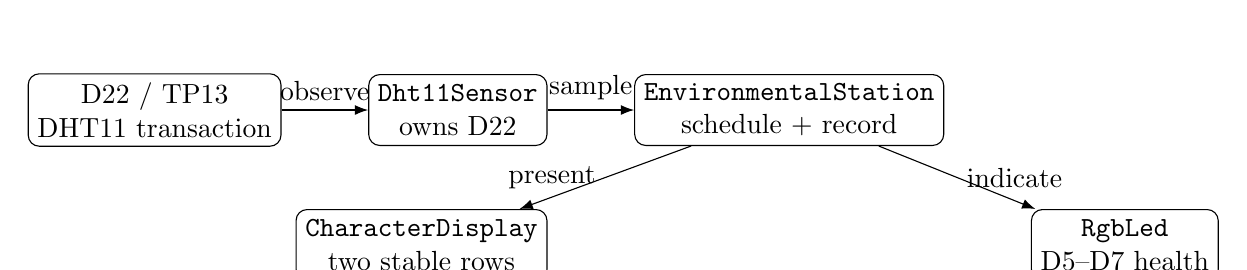
\begin{tikzpicture}[
    node distance=8mm and 11mm,
    box/.style={draw,rounded corners,minimum height=9mm,align=center},
    >=Latex]
  \node[box] (wire) {D22 / TP13\\DHT11 transaction};
  \node[box,right=of wire] (sensor) {\texttt{Dht11Sensor}\\owns D22};
  \node[box,right=of sensor] (station) {\texttt{EnvironmentalStation}\\schedule + record};
  \node[box,below left=of station] (lcd) {\texttt{CharacterDisplay}\\two stable rows};
  \node[box,below right=of station] (health) {\texttt{RgbLed}\\D5--D7 health};
  \draw[->] (wire) -- node[above]{observe} (sensor);
  \draw[->] (sensor) -- node[above]{sample} (station);
  \draw[->] (station) -- node[left]{present} (lcd);
  \draw[->] (station) -- node[right]{indicate} (health);
\end{tikzpicture}
\end{center}

\texttt{EnvironmentalStation} receives an explicit non-owning
\texttt{ClimateSensor} relationship. During \texttt{initialize()} it validates
the period and freshness policy, then initializes the sensor. Failure rolls
the sensor back. Repeated initialization does not reacquire it. Shutdown
releases the sensor, clears the schedule and record, and is idempotent; the
destructor repeats this cleanup safely.

The LCD and RGB evidence are owned by the sketch because they are presentation
choices, not part of the station's decision engine. Setup therefore acquires
in dependency order and rolls back in reverse order:

\begin{enumerate}
  \item sensor and station;
  \item LCD;
  \item RGB evidence;
  \item initial blank/fault-safe presentation.
\end{enumerate}

\section{The deterministic record contract}

\begin{tabularx}{\linewidth}{@{}l X@{}}
\toprule
Field & Meaning\\
\midrule
\texttt{sample} & temperature, humidity, observation time, and exact sample state\\
\texttt{health} & starting, healthy, sensor fault, stale, or timing fault\\
\texttt{sensorStatus} & transport/update status without replacing sample detail\\
\texttt{recordedAt} & caller time at which the station recorded the observation\\
\texttt{sequence} & monotonically increasing record number since initialize/reset\\
\bottomrule
\end{tabularx}

The first \texttt{update(now)} is due immediately. After a record, the next
deadline is \(\texttt{now}+\texttt{samplePeriod}\). An early update is a no-op.
A late update takes one observation and schedules from the supplied time; it
does not burst through missed transactions. This prevents a blocked sensor
from turning one late loop into a long catch-up loop.

\texttt{recordReady} is an event snapshot. It is true only for the update that
created a record and remains readable until the next update. The record itself
remains stable between deadlines. Unsigned time works across
\texttt{millis()} rollover while distances remain within the half-range.
Ambiguous reverse time becomes \texttt{TimingFault} and cancels the deadline
until explicit reset.

\begin{lstlisting}[style=adkcpp]
void loop ()
{
    const adk::TimePoint             now      (millis ());
    const adk::Status                status   = station.update (now);
    const adk::EnvironmentalSnapshot evidence = station.snapshot ();

    if (evidence.recordReady)
    {
        presentRecord (evidence.record);
    }

    showHealth (evidence.record.health, status);
    display.update (now);
}
\end{lstlisting}

\section{Parts, wiring, and current}

\begin{tabularx}{\linewidth}{@{}l l X@{}}
\toprule
Quantity & Part & Requirement\\
\midrule
1 & Mega 2560 & USB powered\\
1 & DHT11 & exact bare part or documented module identified\\
1 & 16x2 HD44780 LCD & 5\,V-compatible module, 4-bit interface\\
1 & 10\,k\(\Omega\) potentiometer & LCD contrast between 5\,V and GND\\
1 & DATA pull-up & value required by identified sensor; omit when module supplies it\\
1 & common-cathode RGB LED & three known channel pins plus common cathode\\
3 & 330\,\(\Omega\) resistors & one per RGB channel\\
1 & LCD backlight resistor & only if the identified module does not include one\\
1 & multimeter & continuity and rail checks\\
\bottomrule
\end{tabularx}

\begin{figure}[ht]
  \centering
  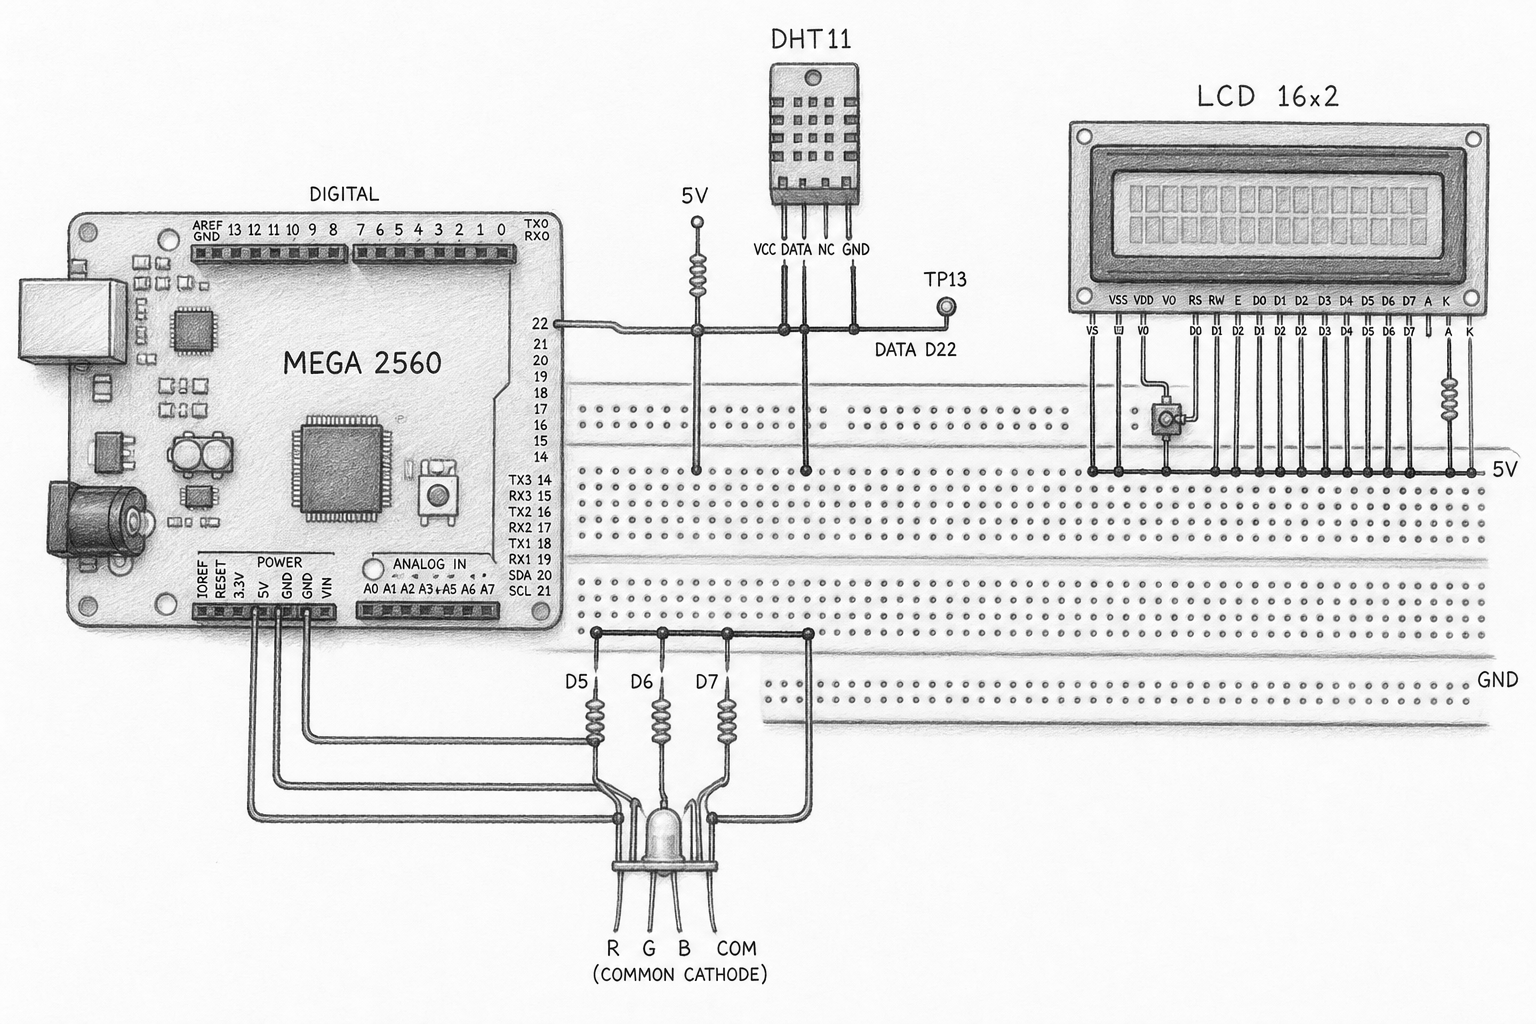
\includegraphics[width=0.96\linewidth]{015-environmental-station-pencil.png}
  \caption{Pencil orientation of the Mega, DHT11, LCD, RGB health indicator,
  and TP13. It is not an authoritative schematic. Alternative text: Mega D22
  reaches DHT11 DATA and TP13; a 16x2 LCD uses a separate six-wire 4-bit
  interface; D5, D6, and D7 each reach one resistor-limited RGB channel; all
  parts share 5\,V and GND, and DHT11 NC remains open.}
\end{figure}

\begin{tabularx}{\linewidth}{@{}l l X@{}}
\toprule
Endpoint & Connection & Evidence\\
\midrule
DHT11 VDD/GND & Mega 5\,V/GND & rail measurement at the sensor\\
DHT11 DATA & D22, pull-up if required & TP13 pulse transaction\\
DHT11 NC & no connection & continuity check while unpowered\\
LCD RS, E & D30, D31 & command/data strobes\\
LCD D4--D7 & D32--D35 & 4-bit data path\\
LCD RW & GND & write-only operation\\
LCD VO & contrast potentiometer wiper & readable cells after adjustment\\
RGB R/G/B & D5/D6/D7 through 330\,\(\Omega\) each & health cadence\\
RGB common cathode & GND & shared return\\
\bottomrule
\end{tabularx}

Use the actual LED forward voltages to calculate each channel current:

\[
I=\frac{V_{\mathrm{rail}}-V_f}{R}.
\]

Record each value and the worst simultaneous total. Do not infer current from
brightness. If the LCD module exposes a raw backlight LED, use its documented
series resistance rather than assuming resistance is on the board.

\section{Predict, observe, interpret}

\subsection{Acquisition evidence}

\textbf{Predict:} after all resources initialize, the LCD shows a starting
record and the RGB indicator begins the slow starting cadence. If any claim
fails, the LCD is blanked and all RGB channels turn off.

\textbf{Observe:} power the checked circuit. Watch the complete startup
sequence rather than a single final LED state. Confirm that the first numbered
record appears only after the scheduled observation.

\textbf{Interpret:} the sequence proves that software acquired its objects and
advanced the loop. It does not prove electrical output levels or climate
accuracy.

\subsection{Healthy and fault records}

\textbf{Predict:} a valid fresh sample displays temperature/humidity and a
record number while the indicator gives the healthy cadence. A timeout,
checksum failure, invalid range, or stale sample remains visible as a named
fault record; old valid values are not relabeled as new.

\textbf{Observe:} record both LCD rows and the LED cadence. With power removed,
disconnect only DATA to create a controlled transport fault, recheck the
wiring, then power again. Restore DATA only with power removed.

\textbf{Interpret:} a fault record demonstrates explicit uncertainty. A
healthy record demonstrates accepted digital data, not calibration against a
reference instrument.

\subsection{Electrical safe state}

\textbf{Predict:} after commanded shutdown, D22 and every owned display or RGB
pin reach their documented inactive/high-impedance state. The LCD and RGB LED
are off.

\textbf{Observe:} invoke the lesson shutdown path, then measure the named pins
relative to GND. Separately remove USB power and confirm the circuit is
de-energized.

\textbf{Interpret:} pin measurements support the safe-state claim. Merely
seeing a dark LED does not: a reversed or failed LED can also appear dark.

\section{Host replay and CLI workflow}

The host test injects a recorded sensor rather than waiting for a room to
change. Its trace covers immediate first sampling, exact deadlines, early
no-ops, late updates without catch-up bursts, healthy/fault/stale recovery,
initialization rollback, restart, destruction, rollover, ambiguous time, and
byte-for-byte replay.

\begin{verbatim}
make test-environmental-station
make test-sanitize
make compile-Lesson015EnvironmentalStation
make size-Lesson015EnvironmentalStation
make lesson-015
make lessons-check
make upload-Lesson015EnvironmentalStation PORT=/dev/ttyACM0
make monitor PORT=/dev/ttyACM0
\end{verbatim}

Serial monitoring is optional supporting context. The LCD, RGB cadence, and
TP13 remain the required evidence paths.

The canonical Mega 2560 build uses 14,134 bytes of flash and 912 bytes of
static RAM with the current Arch Arduino AVR toolchain. These are compile-size
measurements, not runtime-stack or physical-current measurements.

\section{Diagnosis}

\begin{tabularx}{\linewidth}{@{}p{0.22\linewidth} X X@{}}
\toprule
Observation & Likely boundary & Next check with power removed\\
\midrule
No LCD, no RGB sequence & acquisition or supply & rail polarity, shorts, pin claims\\
RGB healthy, LCD blank & presentation & LCD pin 1 orientation, VO contrast, RW to GND\\
Fault record, TP13 quiet & sensor power/DATA & sensor identity, pull-up, D22 continuity\\
Fault record, TP13 active & transport/validation & timing capture, checksum/range state\\
Same sequence repeats & scheduling loop stalled & visible cadence and caller time path\\
Plausible but wrong values & environment or accuracy & compare with a documented reference; do not recalibrate by guess\\
LED dark after shutdown & inconclusive alone & measure D5--D7 and D22 relative to GND\\
\bottomrule
\end{tabularx}

\section{Exercises}

\begin{enumerate}
  \item Predict the record sequence and deadlines for updates at 0, 1999,
        2000, 9000, and 9001\,ms with a 2000\,ms period. Explain the lack of
        catch-up records.
  \item Extend a recorded host trace with checksum failure, stale sample, and
        recovery. List every expected health value before running it.
  \item Design two LCD rows that fit exactly 16 columns and retain sample state,
        age, and sequence. Explain which numeric detail you omit and why.
  \item Explain why the station owns the sensor lifecycle but does not own the
        presentation objects.
  \item Measure the RGB channel currents and compare them with the calculated
        values. Record rail voltage, \(V_f\), resistor value, and uncertainty.
  \item Inject a display failure in a host fake. Specify the station record
        that must remain preserved even though presentation failed.
\end{enumerate}

\section{Bench acceptance record}

\begin{tabularx}{\linewidth}{@{}l X@{}}
\toprule
Item & Record\\
\midrule
Board and USB supply & \blank{0.70\linewidth}\\
DHT11 part/module source & \blank{0.62\linewidth}\\
LCD part/source and backlight limit & \blank{0.52\linewidth}\\
Measured 5\,V rail & \blank{0.68\linewidth}\\
RGB resistors and channel currents & \blank{0.53\linewidth}\\
Unpowered continuity/polarity check & \checkbox\ pass \quad \checkbox\ stop\\
Startup/acquisition sequence & \blank{0.57\linewidth}\\
Healthy record and cadence & \blank{0.58\linewidth}\\
Controlled DATA fault record & \blank{0.55\linewidth}\\
Reset/recovery observation & \blank{0.59\linewidth}\\
Shutdown pin measurements & \blank{0.57\linewidth}\\
Power-removed observation & \blank{0.59\linewidth}\\
Instrument, date, reviewer & \blank{0.61\linewidth}\\
Deviation or stop reason & \blank{0.63\linewidth}\\
\bottomrule
\end{tabularx}

\evidencebox{\textbf{Release status: host verified; physical acceptance open.}
Compilation, host replay, generated PDF, and firmware size are not physical
evidence. Do not mark this lesson hardware accepted until the completed record
contains measured startup, normal, fault, reset, shutdown, and power-removed
observations on the named Mega 2560 circuit.}

\section{Further reading}

\begin{itemize}
  \item Arduino Mega 2560 Rev3 documentation:
        \url{https://docs.arduino.cc/hardware/mega-2560/}
  \item DHT11 product documentation from the exact identified manufacturer or
        module supplier
  \item HD44780U controller datasheet from Hitachi/Renesas
  \item ADK development, testing, safety, and PDF policies in the repository
\end{itemize}

\end{document}
